% Template for ICIP-2026 paper; to be used with:
%          spconf.sty  - ICASSP/ICIP LaTeX style file, and
%          IEEEbib.bst - IEEE bibliography style file.
% --------------------------------------------------------------------------
\documentclass{article}
\usepackage{spconf,amsmath,amssymb,graphicx}
% Bold italic math symbols (vectors/matrices)
\usepackage{bm}
% Chinese support (XeLaTeX)
\usepackage{fontspec}
\usepackage{xeCJK}
% Hyperlinks for references (load near end of preamble)
\usepackage{hyperref}
\hypersetup{
  colorlinks=true,
  linkcolor=blue,
  citecolor=blue,
  urlcolor=blue,
  bookmarksnumbered=true,
  pdfstartview=FitH
}
% Prefer Noto CJK fonts; fallback to WenQuanYi if unavailable.
\IfFontExistsTF{Noto Serif CJK SC}{
  \setCJKmainfont{Noto Serif CJK SC}
}{
  \IfFontExistsTF{Noto Sans CJK SC}{
    \setCJKmainfont{Noto Sans CJK SC}
  }{
    \IfFontExistsTF{WenQuanYi Zen Hei}{
      \setCJKmainfont{WenQuanYi Zen Hei}
    }{
      \IfFontExistsTF{AR PL UMing CN}{
        \setCJKmainfont{AR PL UMing CN}
      }{
        % Last resort: let XeTeX try system default (may still warn).
        \setCJKmainfont{SimSun}
      }
    }
  }
}
\IfFontExistsTF{WenQuanYi Zen Hei Mono}{\setCJKmonofont{WenQuanYi Zen Hei Mono}}{}
% Better Chinese line breaking
\XeTeXlinebreaklocale "zh"
\XeTeXlinebreakskip = 0pt plus 1pt

% Example definitions.
% --------------------
\def\x{{\bm x}}
% NOTE: Avoid overriding \L (reserved command in LaTeX). Use \mathcal{L} directly.

% Title.
% ------
\title{CoReGate:基于反事实门控融合的多模态情感分析}
%
% Single address.
% ---------------
\name{Author(s) Name(s)\thanks{Thanks to XYZ agency for funding.}}
\address{Author Affiliation(s)}
%
% For example:
% ------------
%\address{School\\
%	Department\\
%	Address}
%
% Two addresses (uncomment and modify for two-address case).
% ----------------------------------------------------------
%\twoauthors
%  {A. Author-one, B. Author-two\sthanks{Thanks to XYZ agency for funding.}}
%	{School A-B\\
%	Department A-B\\
%	Address A-B}
%  {C. Author-three, D. Author-four\sthanks{The fourth author performed the work
%	while at ...}}
%	{School C-D\\
%	Department C-D\\
%	Address C-D}
%
\begin{document}
%\ninept
%
\maketitle
%
\begin{abstract}
多模态情感分析中,文本通常更稳定,而音频与视觉在噪声、缺失或与文本语义冲突时可能引入不可靠证据,使直接融合产生误差放大。本文提出 CoReGate(Counterfactual Reliability-Gated Fusion),将非语言模态建模为对文本预测的增量修正:通过多分支预测显式估计音频与视觉带来的边际贡献,并学习样本级可靠性门控以进行选择性特征注入,从而在非语言模态不可靠时抑制其不确定贡献并提升预测稳定性。我们在 CMU-MOSI 与 CMU-MOSEI 上进行评估,结果表明该方法在标准评测指标上具有竞争力,并在缺失模态压力测试下表现出更好的鲁棒性。
\end{abstract}
%
\begin{keywords}
Multimodal sentiment analysis, counterfactual contribution, reliability gating, robust fusion
\end{keywords}
%
\section{INTRODUCTION}
\label{sec:intro}

多模态情感分析(Multimodal Sentiment Analysis, MSA)旨在综合文本、音频与视觉等线索,对用户表达的情感强度或极性进行预测,是人机交互与多模态理解中的基础任务之一~\cite{zhu2024review}。尽管融合能够引入互补信息,但在真实场景中非语言模态往往更易受采集条件、背景噪声、遮挡与缺失等因素影响,并可能与文本语义发生冲突(例如讽刺或反语),从而使“直接融合”既可能带来收益,也可能放大误差并导致性能不稳定~\cite{williams2018dnn,wang2022cross}。如 Fig.~\ref{fig:intro_motivation} 所示,当音频与视觉存在噪声或与文本语义相悖时,简单融合容易引入不可靠证据并放大预测偏差。

\begin{figure}[t]
  \centering
  \includegraphics[width=0.98\linewidth]{figures/fig1}
  \caption{Motivation for robust multimodal fusion. When audio and vision are noisy or semantically conflicting with text (e.g., sarcasm), naive fusion may amplify prediction errors.}
  \label{fig:intro_motivation}
\end{figure}

\begin{figure*}[t]
  \centering
  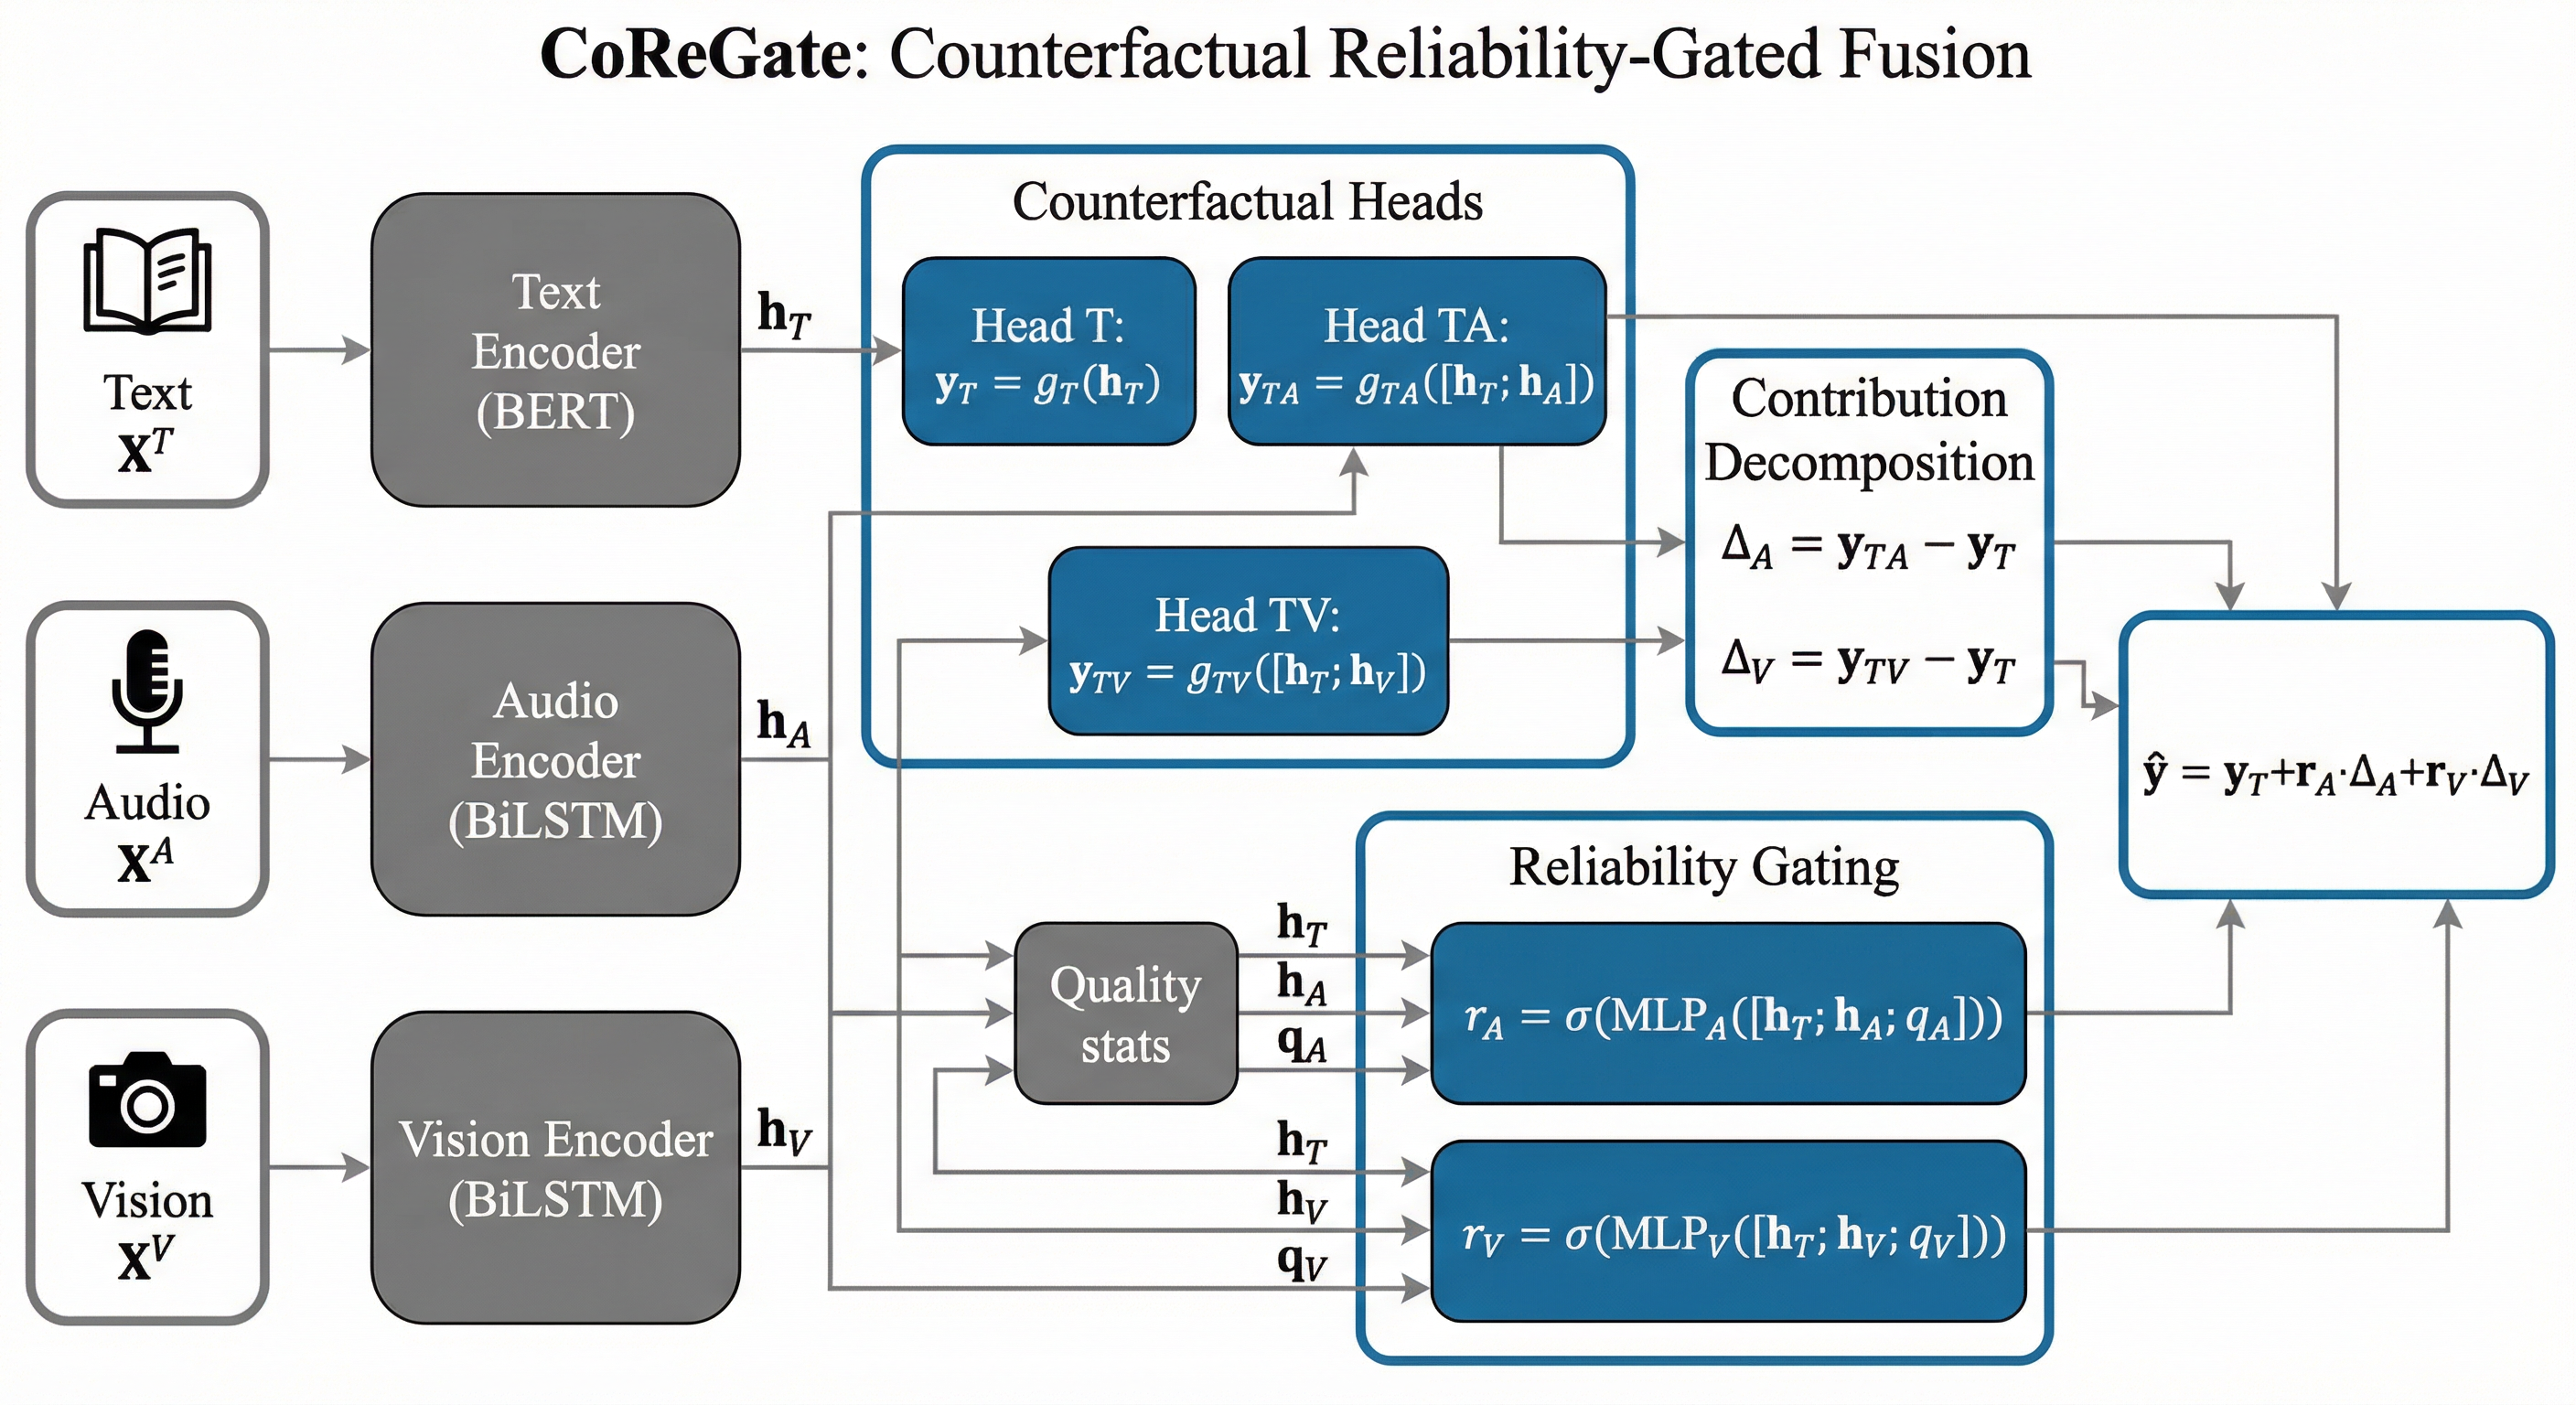
\includegraphics[width=0.98\textwidth]{figures/fig2}
  \caption{Overview of CoReGate. Text is treated as a backbone predictor. Audio and vision provide marginal increments (\(\Delta_{\mathrm{A}},\Delta_{\mathrm{V}}\)) estimated by counterfactual heads and injected by sample-wise reliability gates (\(r_{\mathrm{A}},r_{\mathrm{V}}\)).}
  \label{fig:framework}
\end{figure*}

现有研究主要从融合算子、表示学习与鲁棒性建模等角度推进 MSA,可粗略归纳为以下几类。首先,在\textbf{融合范式}上,经典方法从输入级特征拼接,到中间表征融合与决策级加权等,系统探索了不同“融合介入层级”的取舍~\cite{williams2018dnn,williams2018recognizing};也有研究进一步从\emph{主导模态补全/引导融合}出发缓解模态贡献不均衡问题~\cite{huang2023dominant}。其次,在\textbf{显式交互建模}上,张量融合及其低秩近似通过外积或分解形式刻画高阶跨模态交互,通常伴随更高的表示维度或计算代价~\cite{zadeh2017tensor,liu2018efficient};面向序列数据的建模进一步引入跨时间的交互与记忆机制,并结合图结构建模以捕获时序依赖、异步交互或结构关系~\cite{zadeh2018memory,zadeh2018multimodal,hu2024graph}。

与此同时,\textbf{表示学习}路线通过共享与私有或模态不变与模态特异分解来缓解模态差异与冗余,并结合自监督或多任务信号增强模态特异信息~\cite{tsai2019learning,hazarika2020misa,yu2021learning}。近年来,\textbf{文本主导的跨模态增强}受到关注,倾向于以文本为语义锚点,将非语言线索注入文本表征以适配未对齐场景~\cite{wang2022cross,wang2023tetfn,li2025caetfn};此外也有工作从对比去噪、不完整模态学习与多级对比学习等角度提升模型对噪声与缺失的鲁棒性~\cite{wang2025contrastive,jiang2025boosting,zhuang2025multi,zhu2024review}。在更细粒度的方面级多模态情感分析中亦有相关探索~\cite{wang2024dual}。

尽管上述方法有效提升了平均性能,但在“强文本、弱且不稳定的非语言模态”这一现实设置下,一个核心困难仍未被充分解决:当音频与视觉噪声、缺失或与文本冲突时,融合模型往往缺少对非语言信息\emph{何时以及在多大程度上应当被利用或抑制}的可控机制,因而容易将不可靠证据注入预测并放大误差~\cite{williams2018dnn,zadeh2017tensor,zadeh2018memory,wang2022cross,wang2023tetfn,wang2025contrastive,jiang2025boosting}。因此,我们希望构建一种以文本为主干、对非语言信息进行可解释且可控的增量注入方式,使模型在非语言模态噪声、缺失或冲突等情形下仍能保持更稳定的预测。

为此,我们提出 CoReGate(Counterfactual Reliability-Gated Fusion),将非语言模态建模为对文本预测的\emph{增量修正}:分别学习文本分支、文本+音频分支与文本+视觉分支的预测,并通过\textbf{反事实贡献分解}(即“加入某一模态前后预测的差分”)显式刻画该模态带来的边际修正;随后由样本级可靠性门控根据表征线索与模态质量统计,选择性注入这些修正,从而在音频与视觉噪声、缺失或与文本冲突时抑制不可靠信息。

我们的主要贡献总结如下:
\begin{itemize}
  \item 提出一种基于反事实贡献分解与可靠性门控的稳健融合框架,将非语言模态显式建模为对文本预测的增量修正。
  \item 在 CMU-MOSI 与 CMU-MOSEI 上的实验表明,所提方法在标准评测与缺失模态压力测试下均具有稳定的性能与鲁棒性优势。
\end{itemize}

\section{PROPOSED METHOD}
\label{sec:method}

本节提出一种基于反事实贡献分解(counterfactual contribution decomposition)与可靠性门控(reliability gating)的稳健融合框架。我们以文本预测为主干,并将音频与视觉视作对文本的\emph{增量证据}:模型输出三个分支预测(\(\mathrm{T}\)、\(\mathrm{TA}\)、\(\mathrm{TV}\)),由此构造边际贡献,再通过样本级门控选择性注入贡献项,从而在噪声或冲突模态存在时仍保持稳健。

如 Fig.~\ref{fig:framework} 所示,我们先分别编码三模态得到 \(\bm{h}_{\mathrm{T}},\bm{h}_{\mathrm{A}},\bm{h}_{\mathrm{V}}\),并训练三个分支预测器得到 \(y_{\mathrm{T}},y_{\mathrm{TA}},y_{\mathrm{TV}}\)。由此计算边际贡献 \(\Delta_{\mathrm{A}},\Delta_{\mathrm{V}}\),再由门控网络结合表征线索与质量统计 \((\bm{q}_{\mathrm{A}},\bm{q}_{\mathrm{V}})\) 预测可靠性系数 \(r_{\mathrm{A}},r_{\mathrm{V}}\),最终在输出层对增量进行选择性注入,以在非语言模态不可靠时抑制不可靠增量。

\subsection{Problem Formulation}
\label{ssec:form}

我们将三模态输入表示为序列特征 \(\bm{X}^{(\mathrm{T})},\bm{X}^{(\mathrm{A})},\bm{X}^{(\mathrm{V})}\)。用 \(\mathrm{T},\mathrm{A},\mathrm{V}\) 作为模态索引,并记 \(E_m(\cdot)\) 为模态 \(m\in\{\mathrm{T},\mathrm{A},\mathrm{V}\}\) 的编码器,输出句级向量 \(\bm{h}_m = E_m(\bm{X}^{(m)})\)。对于任意模态子集 \(\mathcal{S}\subseteq\{\mathrm{T},\mathrm{A},\mathrm{V}\}\),我们定义分支预测为

\begin{equation}
y_{\mathcal{S}} = g_{\mathcal{S}}\!\left(f_{\mathcal{S}}\big(\{\bm{h}_m\}_{m\in \mathcal{S}}\big)\right),\quad \mathcal{S}\in\{\mathrm{T},\mathrm{TA},\mathrm{TV}\}.
\end{equation}
其中 \(f_{\mathcal{S}}(\cdot)\) 为分支 \(\mathcal{S}\) 的融合算子(本文采用拼接并接一层感知机实现),\(g_{\mathcal{S}}(\cdot)\) 为对应的回归头,输出标量预测 \(y_{\mathcal{S}}\)。
在下文中,我们以 \(y_{\mathrm{T}}\) 作为文本主干输出,其余分支用于构造可控且便于分析的增量贡献。

\subsection{Encoders and Representations}
\label{ssec:enc}
我们将文本、音频与视觉分别表示为序列输入,其中音频与视觉允许与文本\emph{未对齐},并通过有效长度或掩码处理补零填充的时间步。文本编码器采用预训练语言模型提取句级表征(取 \texttt{[CLS]} 对应的隐向量作为 \(\bm{h}_{\mathrm{T}}\))。对音频与视觉,我们使用轻量时序编码器对帧级特征进行上下文建模,得到序列隐状态后再聚合为句级表示 \(\bm{h}_{\mathrm{A}},\bm{h}_{\mathrm{V}}\)。聚合阶段采用文本引导的注意力池化(以文本表征为查询,从未对齐的音频与视觉序列中选择与语义相关的时间片)。上述 \(\bm{h}_{\mathrm{T}},\bm{h}_{\mathrm{A}},\bm{h}_{\mathrm{V}}\) 将用于三分支预测与后续的可靠性门控。

\subsection{Counterfactual Contribution Decomposition}
\label{ssec:cf}

现有融合方法多依赖隐式注意力或表示对齐来平衡模态,缺少可操作、可量化的“模态贡献”定义;在仅有总体情感标签监督的条件下,模型也难以稳定学习何时应信任或抑制某模态。我们将“模态贡献”定义为\textbf{在固定其它模态条件下,加入该模态导致预测变化的差分量},从而赋予贡献明确的反事实语义,并可由多分支预测直接估计。

具体地,我们以文本为主干、将音频与视觉视为可选修正信号。设 \(y_{\mathrm{T}}\) 为仅文本预测,\(y_{\mathrm{TA}}\)、\(y_{\mathrm{TV}}\) 分别为文本+音频、文本+视觉预测。定义边际贡献为
\begin{equation}
\begin{aligned}
\Delta_{\mathrm{A}} &= y_{\mathrm{TA}}-y_{\mathrm{T}}, \\
\Delta_{\mathrm{V}} &= y_{\mathrm{TV}}-y_{\mathrm{T}}.
\end{aligned}
\end{equation}
直观地,\(\Delta_{\mathrm{A}}\) 与 \(\Delta_{\mathrm{V}}\) 分别度量音频与视觉对文本预测的净修正。这种分解将“融合增益”拆解为可计算的差分项,使融合从隐式的特征加权转化为对\emph{增量证据}的显式建模;在此基础上,门控机制对贡献项进行样本级选择性注入,从而提升训练稳定性与鲁棒性。

\subsection{Reliability-Gated Fusion}
\label{ssec:gate}

在真实数据中,音频或视觉常受采集条件影响而出现噪声、缺失或与文本语义冲突;若将贡献项一律注入,不可靠模态会将预测系统性带偏。为此,我们为每个样本学习门控系数 \(r_{\mathrm{A}}, r_{\mathrm{V}}\in[0,1]\),以“该贡献是否可信”为准则选择性注入,最终预测写为
\begin{equation}
\hat{y} = y_{\mathrm{T}} + r_{\mathrm{A}}\Delta_{\mathrm{A}} + r_{\mathrm{V}}\Delta_{\mathrm{V}}.
\end{equation}
当某模态不可靠时,较小的门控系数会抑制其增量对最终预测的影响,使输出更接近文本主干预测;当非语言模态提供互补信息时,门控允许其贡献注入以修正输出。为让门控与“可靠性”语义对齐,我们将门控网络建立在\textbf{表征线索}与\textbf{模态质量统计}两类信息之上。由于分支融合采用拼接实现,我们直接以 \(\bm{h}_{\mathrm{T}},\bm{h}_{\mathrm{A}},\bm{h}_{\mathrm{V}}\) 及质量统计构造门控输入向量:
\begin{equation}
\begin{aligned}
\bm{z}_{\mathrm{A}} &= \big[\bm{h}_{\mathrm{T}};\bm{h}_{\mathrm{A}};\bm{q}_{\mathrm{A}} \big], \\
\bm{z}_{\mathrm{V}} &= \big[\bm{h}_{\mathrm{T}};\bm{h}_{\mathrm{V}};\bm{q}_{\mathrm{V}} \big],
\end{aligned}
\end{equation}
并以 MLP 预测门控系数:
\begin{equation}
\begin{aligned}
r_{\mathrm{A}} &= \sigma(\mathrm{MLP}_{\mathrm{A}}(\bm{z}_{\mathrm{A}})), \\
r_{\mathrm{V}} &= \sigma(\mathrm{MLP}_{\mathrm{V}}(\bm{z}_{\mathrm{V}})).
\end{aligned}
\end{equation}
其中 \(\sigma(\cdot)\) 为 Sigmoid。这里 \(\bm{h}_{\mathrm{T}}\) 为文本表征,\(\bm{h}_{\mathrm{A}},\bm{h}_{\mathrm{V}}\) 为与文本相关的音频与视觉上下文表征;\(\bm{q}_{\mathrm{A}},\bm{q}_{\mathrm{V}}\) 为低维的样本级模态质量统计,用于为门控提供可靠性线索。在实现中,我们对每个模态的有效时间步计算帧级特征的 \(L_2\) 范数,并以其均值、标准差与有效比例组成 \(\bm{q}\in\mathbb{R}^{3}\)。

与直接在融合特征上学习权重不同,我们对\textbf{贡献差分}施加门控,使门控更接近“是否相信该模态提供的\emph{增量证据}”。

\begin{table*}[t]
  \centering
\caption{CMU-MOSI 与 CMU-MOSEI 主结果。Acc2/F1 格式为 Has0/Non0(\%)。}
  \label{tab:main}
  \small
  \begin{tabular}{l|ccccc|ccccc}
    \hline
    & \multicolumn{5}{c|}{\textbf{CMU-MOSI}} & \multicolumn{5}{c}{\textbf{CMU-MOSEI}} \\
    \hline
    Models & MAE$\downarrow$ & Corr$\uparrow$ & Acc7$\uparrow$ & Acc2$\uparrow$ & F1$\uparrow$ & MAE$\downarrow$ & Corr$\uparrow$ & Acc7$\uparrow$ & Acc2$\uparrow$ & F1$\uparrow$ \\
    \hline
    EF-LSTM~\cite{williams2018recognizing} & 0.956 & 0.658 & 32.5 & 78.1/79.3 & 78.2/79.4 & 0.593 & 0.689 & 50.0 & 78.2/81.7 & 78.7/81.7 \\
    LF-DNN~\cite{williams2018dnn} & 0.992 & 0.650 & 33.2 & 76.5/77.7 & 76.6/77.9 & 0.557 & 0.728 & 53.1 & \textbf{83.6}/83.7 & \textbf{83.3}/83.1 \\
    TFN~\cite{zadeh2017tensor} & 0.988 & 0.640 & 35.6 & 75.1/76.1 & 75.1/76.2 & 0.565 & 0.725 & 52.7 & 80.4/83.4 & 80.9/83.4 \\
    LMF~\cite{liu2018efficient} & 0.981 & 0.637 & 36.0 & 75.4/76.2 & 75.4/76.3 & 0.562 & 0.739 & 51.5 & 81.8/83.9 & 82.1/83.8 \\
    MFN~\cite{zadeh2018memory} & 0.938 & 0.669 & 35.9 & 77.0/78.9 & 77.6/78.9 & 0.568 & 0.726 & 50.7 & 82.2/84.0 & 82.3/83.8 \\
    MFM~\cite{tsai2019learning} & 0.899 & 0.673 & 37.8 & 78.9/80.2 & 78.8/80.1 & 0.573 & 0.727 & 51.0 & 81.7/83.6 & 82.1/83.6 \\
    Graph-MFN~\cite{zadeh2018multimodal} & 0.886 & 0.693 & 37.6 & 79.6/81.0 & 79.4/80.8 & 0.562 & 0.725 & 52.1 & 83.3/83.4 & 83.1/82.8 \\
    MISA~\cite{hazarika2020misa} & 0.805 & 0.765 & 40.2 & 81.6/83.2 & 81.6/83.3 & 0.547 & 0.759 & 51.9 & 82.8/84.9 & 83.0/84.8 \\
    Self-MM~\cite{yu2021learning} & 0.726 & 0.784 & \textbf{48.0} & 82.5/84.5 & 82.5/84.5 & 0.539 & 0.765 & 52.8 & 74.8/82.0 & 76.0/82.3 \\
    TETFN~\cite{wang2023tetfn} & 0.731 & 0.790 & 45.2 & 80.9/82.8 & 80.9/82.8 & 0.546 & 0.762 & 53.9 & 80.6/85.1 & 81.1/85.1 \\
    MECAM~\cite{wang2025contrastive} & 0.730 & 0.788 & 45.5 & 81.8/83.5 & 81.7/83.4 & 0.535 & 0.770 & 53.8 & 81.8/85.5 & 82.0/85.2 \\
    CENET~\cite{wang2022cross} & 0.739 & 0.789 & 43.6 & 82.1/83.8 & 82.0/83.9 & \textbf{0.529} & \textbf{0.775} & 54.2 & 82.4/85.8 & 82.7/85.6 \\
    \textbf{Ours} & \textbf{0.716} & \textbf{0.794} & 46.9 & \textbf{82.8}/\textbf{84.9} & \textbf{82.7}/\textbf{84.8} & \textbf{0.529} & \textbf{0.775} & \textbf{54.6} & 82.0/\textbf{86.5} & 82.5/\textbf{86.4} \\
    \hline
  \end{tabular}
\end{table*}


\subsection{Training Objective}
\label{ssec:loss}

主任务采用 MAE(L1)回归损失。为稳定各分支学习并避免某些分支失效(例如 \(\mathrm{TA}\) 与 \(\mathrm{TV}\) 学不到有效增量,导致 \(\Delta_{\mathrm{A}},\Delta_{\mathrm{V}}\) 近似噪声),我们在对最终预测 \(\hat{y}\) 施加主监督的同时,对三个分支输出 \(y_{\mathrm{T}},y_{\mathrm{TA}},y_{\mathrm{TV}}\) 施加辅助监督,引入分支损失权重 \(\lambda\ge0\),总损失为
\begin{equation}
\mathcal{L} = \mathcal{L}_{\hat{y}} + \lambda\left(\mathcal{L}_{\mathrm{T}} + \mathcal{L}_{\mathrm{TA}} + \mathcal{L}_{\mathrm{TV}}\right),
\end{equation}
其中 \(\mathcal{L}_{\hat{y}}\) 对最终 \(\hat{y}\) 监督,\(\mathcal{L}_{\mathrm{T}}, \mathcal{L}_{\mathrm{TA}}, \mathcal{L}_{\mathrm{TV}}\) 分别对 \(y_{\mathrm{T}}, y_{\mathrm{TA}}, y_{\mathrm{TV}}\) 监督。该设计保证了贡献项 \(\Delta_{\mathrm{A}},\Delta_{\mathrm{V}}\) 的可学习性:若缺少对 \(\mathrm{TA}\) 与 \(\mathrm{TV}\) 的监督,差分量可能变为噪声,从而削弱门控的有效性。

\section{EXPERIMENTAL RESULTS}
\label{sec:exp}

\subsection{Dataset and Metrics}
\label{ssec:dataset}

我们在 CMU-MOSI 与 CMU-MOSEI 上进行情感回归评估,并遵循数据集的标准划分与既有评测协议。评价指标包括 MAE(越低越好)、相关系数 Corr(越高越好),以及将连续标注离散化后的 Acc7/Acc2/F1。具体地,Acc7 先将预测与标注裁剪到 \([-3,3]\) 并四舍五入到整数等级后计算多分类准确率;二分类 Acc2/F1 以 0 为阈值,其中 Has0 采用 \(\ge 0\) vs. \(<0\)(将 0 视为正类),Non0 则先移除标注为 0 的样本后采用 \(>0\) vs. \(<0\)。所有百分比均以 \% 报告。

\subsection{Implementation Details}
\label{ssec:impl}

我们采用数据集公开的 unaligned 特征(文本、音频与视觉的最大长度分别为 50、500、375)。文本编码器采用 \texttt{bert-base-uncased} 并进行端到端微调;训练采用 Adam 优化器与 MAE(L1)损失,学习率 \(1\times10^{-5}\),权重衰减 \(1\times10^{-4}\),梯度裁剪阈值 2.0,batch size 为 64。我们按验证集 Loss 选择最佳 checkpoint;若连续 8 个 epoch 未提升则早停。实验在 Ubuntu 22.04.5 上进行,使用 PyTorch 2.10.0(CUDA 12.8)与 NVIDIA GeForce RTX 4090(24GB)GPU,CPU 为 AMD EPYC 9654。

\subsection{Evaluation of Our Method}
\label{ssec:main}

表~\ref{tab:main} 汇报了 MOSI 与 MOSEI 上的主结果。总体来看,所提方法在两数据集上均取得了有竞争力的表现,并在多个关键指标上达到最优或并列最优。

在 \textbf{CMU-MOSI} 上,我们在 MAE 与 Corr 上达到最优,同时在二分类 Acc2/F1 的 Has0 与 Non0 两种设置下均取得最佳结果;相较于强基线 CENET~\cite{wang2022cross},MAE 从 0.739 降至 0.716,Corr 从 0.789 提升至 0.794,体现了“以文本为主干、对非语言增量进行门控注入”的收益。需要指出的是,Acc7 的最优结果来自 Self-MM~\cite{yu2021learning},而我们方法在该指标上略低但仍保持较强竞争力。

在 \textbf{CMU-MOSEI} 上,我们在 MAE 与 Corr 上与 CENET~\cite{wang2022cross} 并列最优,并在 Acc7 上取得最优结果;此外,我们在 Acc2/F1 的 Non0(排除中性样本)设置下达到最优。与此同时,Has0 设置下的二分类最优由其它方法获得(例如 LF-DNN~\cite{williams2018dnn}),提示不同评测协议下的优势可能并不完全一致。


\subsection{Ablation and Discussion}
\label{ssec:abl}

表~\ref{tab:ablation} 汇总了消融结果。我们围绕四类关键设计进行对比:\textbf{(i) 反事实贡献分解}(w/o decomposition:不使用差分分解,改为直接融合 \(\hat{y}=g([h_T;h_A;h_V])\) 并保留门控)、\textbf{(ii) 可靠性门控}(w/o gating:将 \(r_{\mathrm{A}}=r_{\mathrm{V}}=1\))、\textbf{(iii) 分支辅助监督}(w/o branch sup:去除对 \(\{y_{\mathrm{T}},y_{\mathrm{TA}},y_{\mathrm{TV}}\}\) 的辅助损失)、以及 \textbf{(iv) 融合输出选择}(t-only:仅使用文本分支 \(y_{\mathrm{T}}\);a-only 与 v-only:保持编码与池化过程不变,仅使用对应预测头输出 \(y_{\mathrm{A}}\) 或 \(y_{\mathrm{V}}\))。

\begin{table}[t]
  \centering
  \caption{Ablation results on CMU-MOSI and CMU-MOSEI. Acc7 is reported in \%.}
  \label{tab:ablation}
  \small
  \setlength{\tabcolsep}{5pt}

  \begin{tabular}{l|ccc}
    \hline
    \multicolumn{4}{c}{\textbf{CMU-MOSI}} \\
    \hline
    Setting & MAE$\downarrow$ & Corr$\uparrow$ & Acc7$\uparrow$ \\
    \hline
    Full (CoReGate) & \textbf{0.7159} & \textbf{0.7944} & \textbf{46.94} \\
    w/o decomposition & 0.7298 & 0.7915 & 45.62 \\
    w/o gating & 0.7211 & 0.7932 & 45.34 \\
    w/o branch sup & 0.7405 & 0.7903 & 44.75 \\
    t-only (\(y=y_{\mathrm{T}}\)) & 0.7370 & 0.7903 & 45.19 \\
    a-only (\(y=y_{\mathrm{A}}\)) & 0.9342 & 0.7019 & 33.38 \\
    v-only (\(y=y_{\mathrm{V}}\)) & 1.4750 & 0.1375 & 15.16 \\
    \hline
  \end{tabular}

  \vspace{2mm}

  \begin{tabular}{l|ccc}
    \hline
    \multicolumn{4}{c}{\textbf{CMU-MOSEI}} \\
    \hline
    Setting & MAE$\downarrow$ & Corr$\uparrow$ & Acc7$\uparrow$ \\
    \hline
    Full (CoReGate) & \textbf{0.5286} & \textbf{0.7746} & \textbf{54.56} \\
    w/o decomposition & 0.5347 & 0.7719 & 54.03 \\
    w/o gating & 0.5318 & 0.7728 & 54.12 \\
    w/o branch sup & 0.5362 & 0.7712 & 53.68 \\
    t-only (\(y=y_{\mathrm{T}}\)) & 0.5422 & 0.7665 & 53.21 \\
    a-only (\(y=y_{\mathrm{A}}\)) & 0.5989 & 0.7129 & 48.92 \\
    v-only (\(y=y_{\mathrm{V}}\)) & 0.6477 & 0.6484 & 47.97 \\
    \hline
  \end{tabular}
\end{table}

从表~\ref{tab:ablation} 可以得到如下结论。首先,\textbf{反事实贡献分解的有效性}:与 w/o decomposition(不做差分分解、改为直接融合)相比,完整模型在 MOSI/MOSEI 上的 MAE 分别降低 \(0.0139/0.0061\),Corr 分别提升 \(0.0029/0.0027\),Acc7 分别提升 \(1.32/0.53\) 个百分点,说明将非语言模态显式建模为“相对文本主干的增量修正”有助于获得更好的整体效果。其次,\textbf{可靠性门控的作用边界}:在标准测试集上,门控带来的收益相对有限(例如 MOSI/MOSEI 上 MAE 分别降低 \(0.0052/0.0032\)),但在缺失模态压力测试下收益显著(见图~\ref{fig:robust_missing}),与门控“抑制不可靠增量注入、提升缺失模态等压力测试下稳健性”的设计目标一致。第三,\textbf{分支辅助监督的重要性}:移除分支监督(w/o branch sup)会带来一致的性能下降,例如 MOSI/MOSEI 上 MAE 分别上升 \(+0.0246/+0.0076\),说明对 \(\mathrm{T},\mathrm{TA},\mathrm{TV}\) 分支的显式约束有助于稳定学习边际贡献,使 \(\Delta_{\mathrm{A}},\Delta_{\mathrm{V}}\) 更可学习。最后,\textbf{融合输出选择与文本主干的必要性}:t-only 在两数据集上显著优于 a-only 与 v-only,表明在该评测设置下单独依赖非文本预测头难以达到同等性能,从而支持“以文本为基线、以音频与视觉为增量修正”的建模策略。

总体而言,CoReGate 将“模态贡献”从隐式权重转化为可计算的反事实差分,并在此基础上通过门控实现对增量证据的选择性注入,使融合过程更便于从贡献角度进行分析与对比。

\subsection{Robustness under Missing Modalities}
\label{ssec:robust}

为验证可靠性门控在缺失模态输入下的作用,我们在测试阶段构造三种缺失设置:将音频置零(missing-A)、将视觉置零(missing-V),以及二者同时置零(missing-A\&V)。在\emph{相同训练权重}下,我们进一步对比门控开启(Gating ON)与强制关闭(Gating OFF,即令 \(r_{\mathrm{A}}=r_{\mathrm{V}}=1\))的差异,以排除重新训练带来的干扰。图~\ref{fig:robust_missing} 给出 MOSI 与 MOSEI 上的 MAE 对比。

\begin{figure}[t]
  \centering
  \includegraphics[width=0.98\linewidth]{figures/fig3}
  \caption{Robustness under missing modalities. We evaluate the same trained checkpoint while masking audio and vision at test time. Reliability gating consistently reduces MAE compared with forcing gates to 1 (Gating OFF), especially when the visual modality is missing.}
  \label{fig:robust_missing}
\end{figure}

可以看到,门控在缺失场景下带来一致的鲁棒性收益:当强制关闭门控时,两数据集在不同缺失设置下的 MAE 均出现上升。例如,在 MOSI 上 missing-V 时 MAE 约增加 \(+0.020\),missing-A\&V 时约增加 \(+0.009\);在 MOSEI 上三种缺失设置下 MAE 均约增加 \(+0.025\sim+0.026\)。这些结果印证了我们的动机:将门控作用于\emph{增量修正}项,有助于在模态缺失等压力测试下抑制不可靠的注入。

\section{CONCLUSION}
\label{sec:conc}

本文针对多模态情感分析中非语言模态易受噪声、缺失与语义冲突影响的问题,提出了 CoReGate(Counterfactual Reliability-Gated Fusion)框架:将音频与视觉建模为对文本预测的增量修正,通过多分支预测显式估计每个模态的边际贡献,并由样本级可靠性门控选择性注入这些修正。在 CMU-MOSI 与 CMU-MOSEI 上的评估表明,所提方法在标准指标上达到了有竞争力的性能(MOSI 上 MAE 降至 0.716、Corr 提升至 0.794,MOSEI 上 Acc7 达到 54.6\%),更重要的是,缺失模态压力测试验证了门控机制的鲁棒性收益,体现了将"模态贡献"从隐式权重转化为可计算反事实差分的优势。未来工作可进一步探索更细粒度的时序级门控、跨模态交互建模以及在更多噪声/缺失/冲突设置下的稳健性验证。

% References
\bibliographystyle{IEEEbib}
\bibliography{strings,refs}

\end{document}
